\documentclass[12pt,a4paper]{article}
% Load required packages
\usepackage{amsmath, amssymb, amsfonts}
\usepackage{listings}
\usepackage{graphicx}
\usepackage{xcolor}
\usepackage{enumitem}
\usepackage[top=1in, bottom=1in, left=1.25in, right=1.25in]{geometry}
\usepackage{xcolor}
\usepackage{fontspec}
\usepackage{xeCJK}
\usepackage{tcolorbox}
\usepackage{setspace}
\usepackage{hyperref}

\tcbuselibrary{listings}
\setstretch{1.4}
% Set Chinese Fonts to Songti TC
\setCJKmainfont{Songti TC}
\hypersetup{
    colorlinks=true, % 啟用顏色鏈接
    linkcolor=blue,  % 內部連結顏色設置為藍色
    filecolor=magenta, % 文件連結顏色
    urlcolor=blue,   % 外部連結顏色設置為青色
    citecolor=blue   % 引用顏色設置為藍色
}
\begin{document}

% 設定文件標題
\title{112-2 小田野自主學習計畫申請計畫書}
\date{}
\maketitle
\noindent 計畫主題:\textbf{腦片小精靈 - 用深度學習來分析和計數腦部神經細胞的重疊情形} \\
申請人姓名:\textbf{杜冠勳} \\
學號:\textbf{B10505044} \\
系級:\textbf{資訊三} \\

\section*{一、團隊基本資料}
\begin{center}
    \begin{tabular}{ | c | c | c | c | }
    \hline
    姓名 & 學號 & 系級 & 聯絡信箱 \\ \hline
    杜冠勳(聯絡窗口) & B10505044 & 資訊三 & b10505044@ntu.edu.tw \\ \hline
    邱士紘 & B10401023 & 醫學三 & b10401023@ntu.edu.tw  \\ \hline
    賴亮昕 & B11902009 & 資訊二 & b11902009@ntu.edu.tw \\ \hline
    
    \end{tabular}
\end{center}

\section*{二、計畫發想}
在神經科學領域,研究腦部細胞間的交互作用對於理解腦部功能至關重要。
尤其是在複雜的腦區,例如 Zona Incerta (ZI) 和 Lateral Habenula (LHb),這些區域的相互作用對於理解神經疾病的發展和治療有著不可忽視的影響。\\
更具體的說,研究者會利用病毒載體螢光蛋白、免疫染色等方式標記特定的細胞,分析這些標記的數量與重疊情形可以給研究者提供許多寶貴的資訊,
例如驗證腦區之間是否存在直接的迴路、某一腦區是否與特定功能有關等等。這些解剖學資訊常常作為神經科學研究計畫的第一批資料,
研究者會根據這些資訊推測腦區的功能、設計後續的光遺傳操弄等動物行為實驗,從而驗證腦區功能,進而對應到人類的腦區,探索現有神經疾病的可能治療方法。\\
然而,傳統的神經細胞計數方法依賴於手動操作,相當耗時。舉例來說,現在研究現場計數重疊細胞的方法是藉由 photoshop,以人眼辨識並且手動標記,這過程顯然費時費力。\\
\\
我們的計劃旨在開發一套方便神經科學研究人員計數細胞的自動化工具,以便更有效地識別和計數在 ZI 和 LHb 腦區中特定標記的神經細胞。
具體來說,我們希望透過自己搭建 CNN 模型,並且寫出簡單易用的使用者介面,來幫助研究人員能夠精確地分析細胞間的交互作用,特別是在壓力等特定條件下的細胞活性變化。
這不僅可以提高實驗數據的效率,而且對於理解複雜的神經迴路和其在神經精神疾病中的角色具有重要意義。\\
附圖為腦片中螢光標記的細胞,我們的任務即是做出能統計圖中紅綠重疊細胞的工具:
\begin{figure}[h]
    \centering
    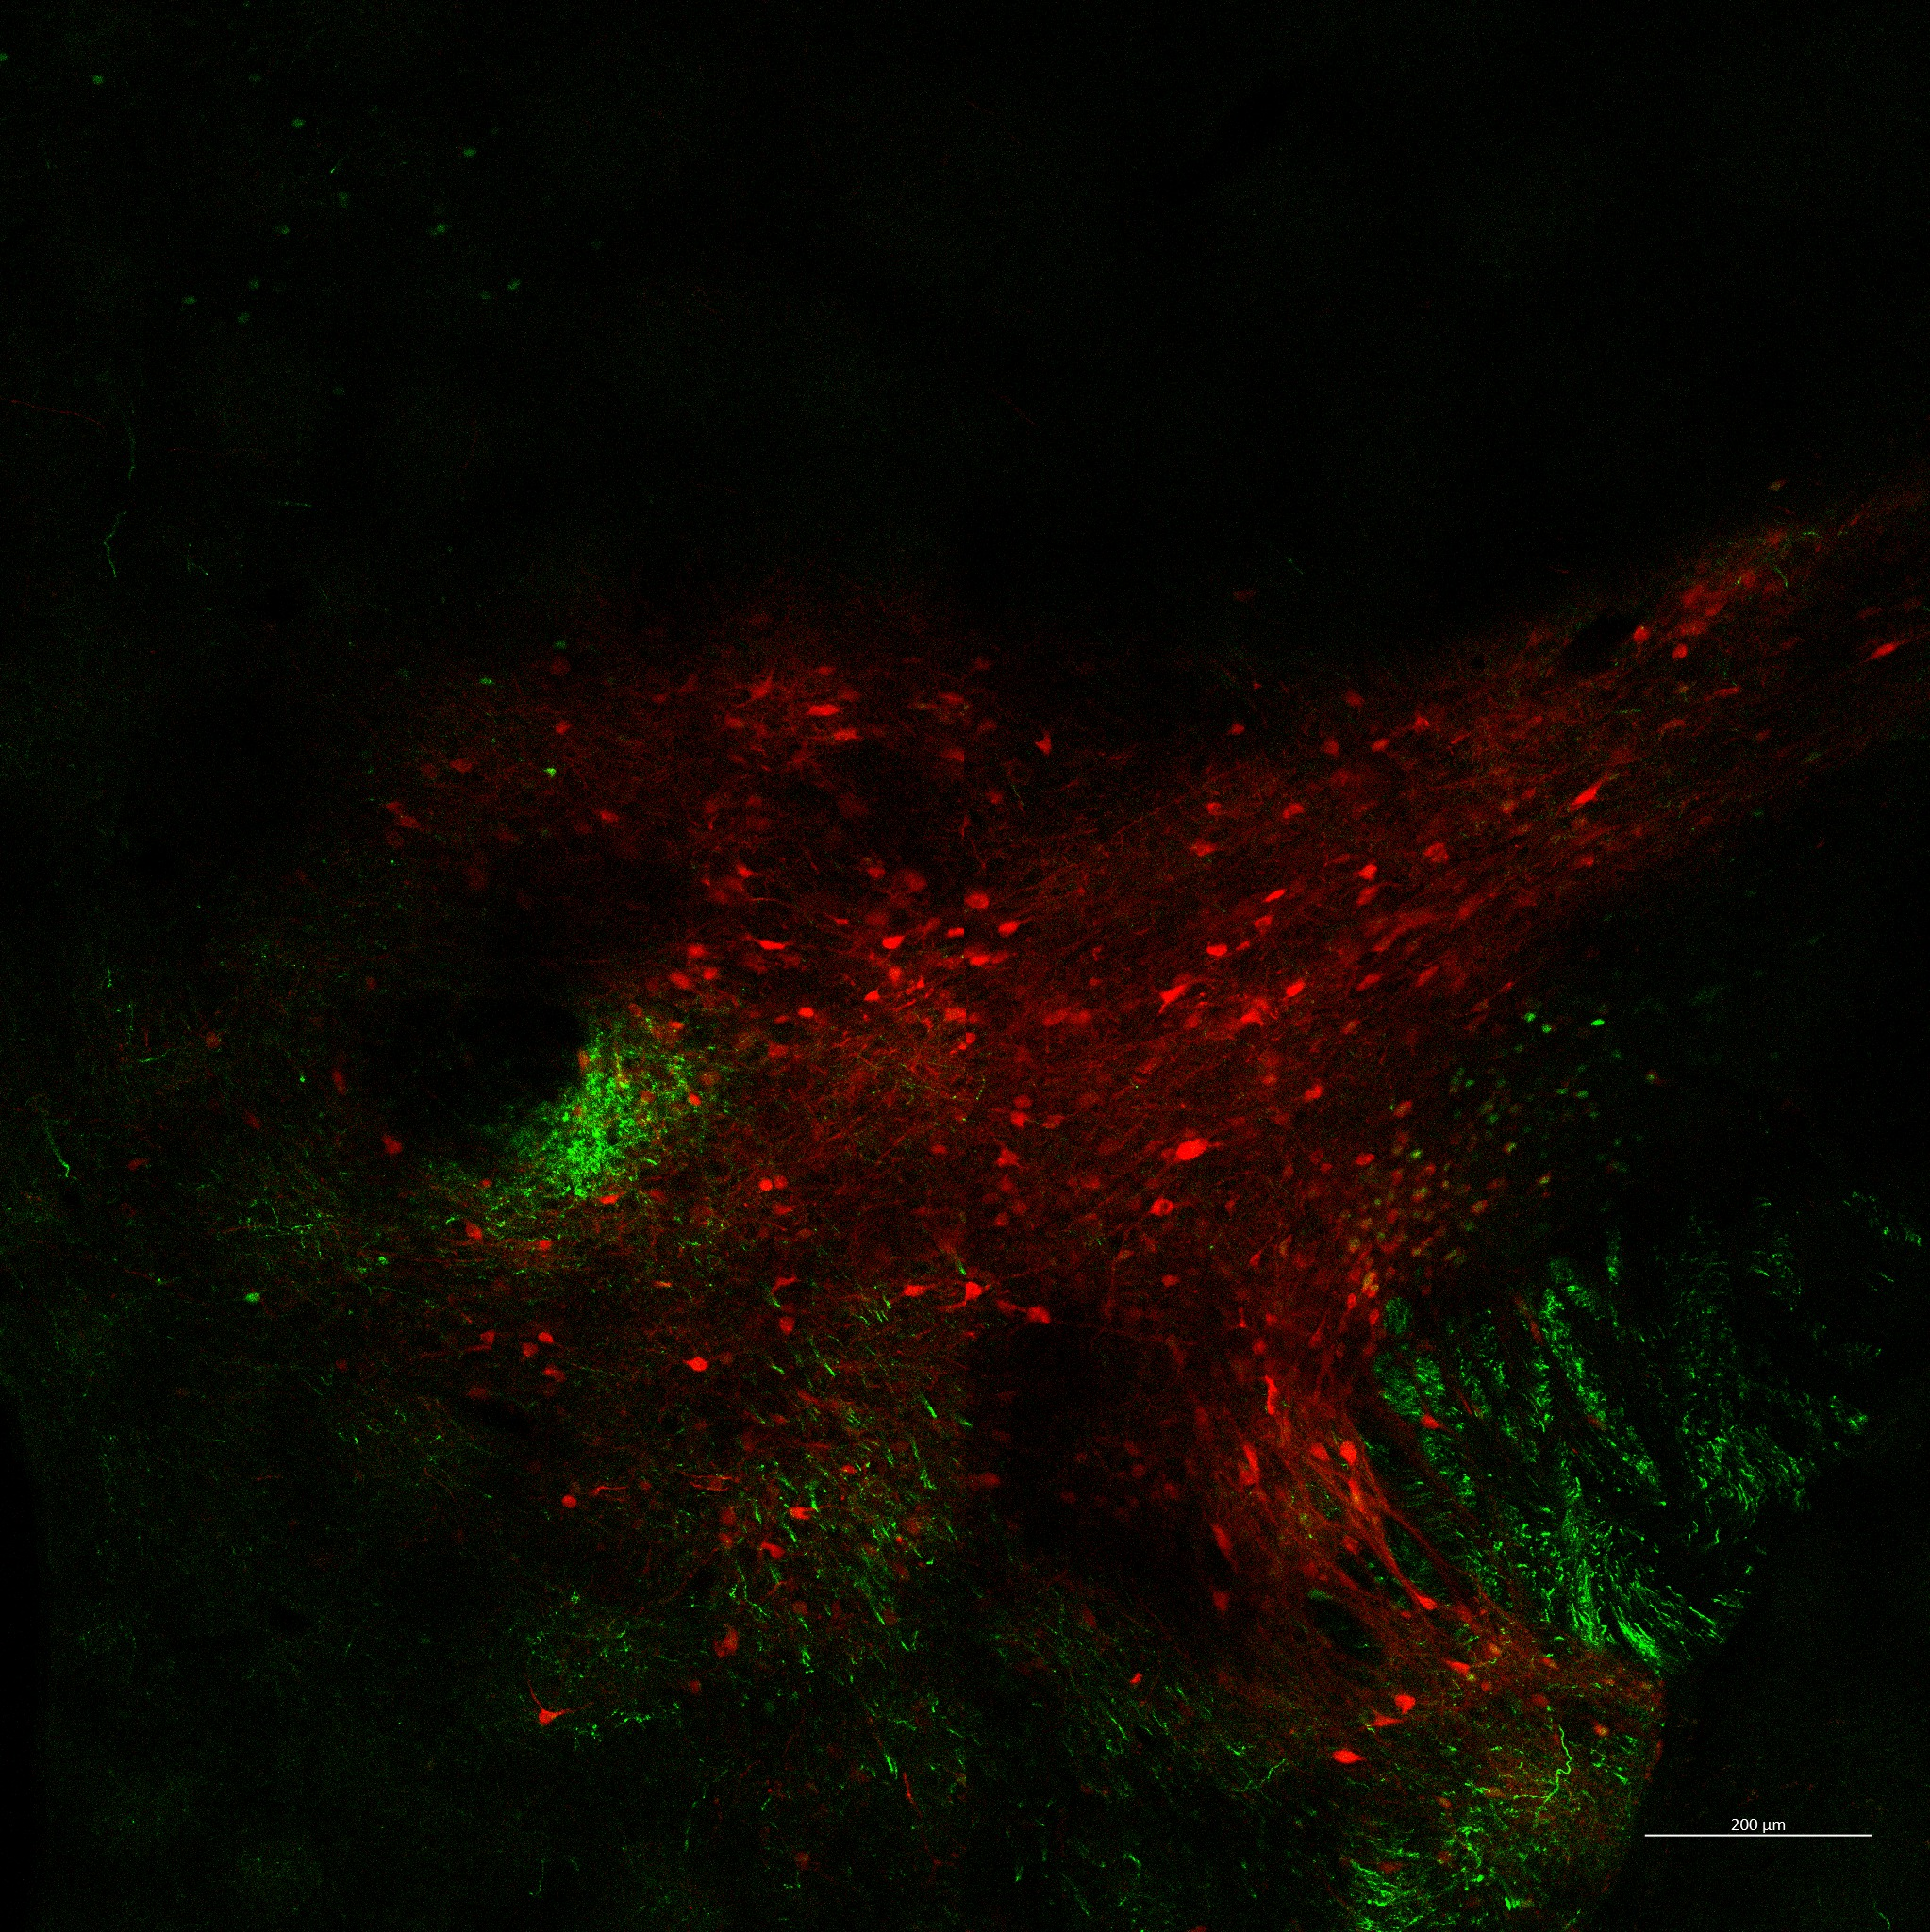
\includegraphics[width=\linewidth]{filename.jpg}
    \caption{圖中不同顏色代表不一樣的神經解剖學或功能意義}
    \label{figure}
    \end{figure}
    
\section*{三、執行方法}

\subsection*{(1) 事前規劃準備}
我們的專案目標是開發一款用於幫助神經科學研究人員計數腦區重疊細胞的 App。
此專案將分為以下幾個關鍵階段:
\begin{enumerate}
    \item \textbf{製作 Dataset}:利用 \textit{labelImg} 這項工具標記提供的腦部影像數據,以製作訓練深度學習模型所需的資料集。醫學系同學將提供相關影像數據,並與資訊系同學合作完成資料標記工作。
    \item \textbf{建構神經網路模型}:使用卷積神經網路 (CNN) 架構來開發能夠準確識別和計數重疊細胞的模型。
    \item \textbf{開發用戶介面 (UI)}:設計一個直觀、易用的用戶介面,讓非技術背景的研究人員也能輕鬆使用這個應用程式。考慮到使用者的操作習慣和需求,進行多次使用者測試和反饋調整。
    \item \textbf{逆向工程}:由於顯微鏡輸出的檔案格式為 \texttt{.czi},我們將探索把 \texttt{.czi} 檔案轉換為 \texttt{.tif} 檔案的方法,以便更好地整合和處理影像數據,對於研究人員來說也會更加方便。
    接著進一步探索從 \texttt{.tif} 檔案中提取出 \texttt{.json} 或 \texttt{.csv} 格式的數據,以製作高品質的資料集。
\end{enumerate}

\subsection*{(2) 初步文獻回顧與市場調查}
我們已經參考了包括 \href{https://www.frontiersin.org/articles/10.3389/fnana.2017.00117/full}{DALMATIAN: An Algorithm for Automatic Cell Detection and Counting in 3D}
 和 
\href{https://www.nature.com/articles/s41598-020-75835-7}{AICellCounter: A Machine Learning‐Based Automated Cell Counting Tool Requiring Only One Image for Training} 等在內的多項論文,
這些研究都提出了優秀的腦片影像分析方法。\\
問題點在於他們的模型雖然 performance 很好,但卻缺乏易用性。
數細胞是費時費力的工作,除了需要準確,還需要容易使用。目前的工具在準確性上或許達標,但大多沒有簡便的取得方式或是方便操作的介面。
我們的創新點在於結合這些技術和一個更加直觀易用的 User Interface,以滿足神經科學領域對於易用性和一定程度正確性的需求。

\subsection*{(3) 計畫過程記錄方式}
我們目前使用 \textit{Notion} 作為主要的項目管理和文檔記錄工具。
通過 \textit{Notion},我們能夠有效地記錄會議紀要、研究進展和相關文檔,並在醫學系與資訊系的團隊成員之間進行有效的知識交流。
此外,我們也定期召開會議來討論專案進展,目前定於每週六下午兩點實體 meeting。


\section*{四、執行期程}

\subsection*{近程目標}
本專案的近程目標聚焦於開發階段的核心活動,具體的月度計劃如下:
\begin{itemize}
    \item \textbf{3月}:完成 Dataset的製作並設計神經網路模型的初步架構,包括從腦部影像中標記數據,以及定義 CNN 的基本參數。
    \item \textbf{4月}:對模型進行細微調整以達到滿意的性能水準,並開始開發 UI。
    \item \textbf{5月}:完成使用者介面,並確保程式在不同平臺能順利運作。
    \item \textbf{6月}:推出 1.0 試用版,提供給台大醫學院實驗室與其他相關研究團體進行小規模測試,收集反饋並進行改進。
    \item \textbf{7、8月}:根據反饋將程式近一步改進,推出 1.1 版。
\end{itemize}

\subsection*{遠程目標}
遠程目標是將這份軟體開源並使之成為廣泛認可和使用的工具,包括:
\begin{itemize}
    \item 在開源平台(如 GitHub)上公開發布程式碼,提供詳細的文檔和使用指南。
    \item 透過社交媒體(如 Reddit)進行宣傳。
    \item 與學術團體合作,收集反饋,並根據用戶需求進行持續更新和改進。
\end{itemize}


\section*{五、預期效益}
本專案目標是提供給團隊成員跨領域的合作經驗,同時對醫學研究領域做出貢獻。具體的預期效益如下:
\begin{itemize}
    \item \textbf{跨學科合作經驗}:通過與醫學系同學的合作,資訊系的成員將有機會深入了解神經科學研究的要點和挑戰,也能了解不同領域的人員看待問題的不同,
    醫學系的同學也更能理解如何與資訊系的人員合作,深度體會機器學習目前能做與不能做的事,
    從而擴展我們的知識面和研究能力。這種合作將強化團隊成員在跨領域溝通和協作方面的能力。
    
    \item \textbf{實踐應用開發經驗}:團隊將獲得寶貴的經驗,包括開發機器學習模型、實踐學術研究到實際應用的轉化,以及開發易用且有效的工具。
    
    \item \textbf{對醫學研究的貢獻}:這份專案我們也希望能對於醫學研究盡一份力,當前端的研究人員能夠少花一些力氣進行細胞計數等重複性工作上的負擔,
    通過自動化這些過程,研究人員能夠將更多精力集中在關鍵的科學發現和創新上。
\end{itemize}

\section*{六、成果展現方式}
本專案的成果將主要通過開源軟體的形式在 GitHub 上進行展示,以便於廣泛地分享和應用。具體的展現方式包括:
\begin{itemize}
    \item \textbf{GitHub Repository}:專案的所有程式、文檔及相關資源將會被托管在 GitHub 上的一個專用資料庫中。這樣不僅便於版本控制和更新,也方便其他研究者和開發者使用與貢獻。

    \item \textbf{詳細的 README 文件}:為了讓用戶能夠輕鬆理解和使用我們的軟體,我們將提供一個詳盡的 README 文件。這個文件將包括安裝指南、使用說明、常見問題解答,以及示例用法。

    \item \textbf{軟體文檔和使用手冊}:除了 README 文件之外,我們還將提供完整的軟體文檔,包括 API References、開發者指南和用戶手冊,以支持各種層次的用戶需求。
\end{itemize}

透過這些方式,我們希望將本專案的成果有效地傳達給科研社群,並促進其在神經科學研究領域的廣泛應用。

\section*{七、預算規劃}
本專案的主要開銷集中在團隊會議和人力時間成本上。具體的預算規劃如下:
\begin{itemize}
    \item \textbf{團隊會議費用}:由於團隊成員每週會在彼此住家附近的咖啡廳進行面對面會議,相關的開銷將包括咖啡廳消費。這是為了提供一個舒適的討論環境,以促進團隊合作和溝通。
    此部分本學期約新台幣\texttt{\$5000}元。 
    \item \textbf{GPU 租用}:要訓練良好的模型需要強大的 GPU,我們預計會租用 \texttt{Colab Pro} 或是類似服務,本學期約新台幣\texttt{\$3000}元。
    \item \textbf{人力時間成本}:雖然專案成員不會直接獲得金錢報酬,但時間和努力投入是重要的非直接成本。團隊成員將投入大量時間於寫程式、實驗設計、數據分析和文檔撰寫等工作。
    \item \textbf{其他潛在成本}:雖然目前專案主要依賴學校提供的資源,如實驗設備和軟體,但可能會有一些意外的小額支出,例如軟體授權續訂或實驗周邊工具,初估本學期約 \texttt{\$2000}。
\end{itemize}
總計本學期花費約新台幣 \$10000 元。
\end{document}
